\documentclass[11pt,a4paper]{article}
\usepackage[top=2.5cm, bottom=2cm, left=2cm, right=2cm]{geometry}
\usepackage{amsmath}
\usepackage{tikz}
\usepackage{circuitikz}
\usepackage{epigraph}
\usepackage{hyperref}
\usepackage{multirow}
%\usepackage[demo]{graphicx}
\usepackage{caption}
\usepackage{subcaption}
\setcounter{secnumdepth}{5}
\usepackage{chngcntr}
\counterwithin{figure}{section}
\counterwithin{table}{section}
\usepackage{multirow}
\setcounter{tocdepth}{5}


\renewcommand\epigraphflush{flushright}
\renewcommand\epigraphsize{\normalsize}
\setlength\epigraphwidth{0.7\textwidth}

\usepackage{color}
\definecolor{titlepagecolor}{cmyk}{1,.0,0.0,.50}
\definecolor{scolour}{cmyk}{1,.0,0.0,.85}
\definecolor{sscolour}{cmyk}{1,.0,0.0,.75}
\definecolor{ssscolour}{cmyk}{1,.0,0.0,.65}
\definecolor{paracolour}{cmyk}{1,.0,0.0,.55}

\usepackage{amsfonts}
%\DeclareFixedFont{\titlefont}{T1}{ams}{b}{sc}{0.5in}

% Added 
\usepackage{fancyhdr}
\pagestyle{fancy}
\lhead{MTRX3700}
\rhead{Group COOLNAME}
\cfoot{\thepage}
\renewcommand{\headrulewidth}{0.4pt}
\renewcommand{\footrulewidth}{0.4pt}
\renewcommand{\thepage}{\roman{page}}
\usepackage{indentfirst}           %remove if we dont want to indent
\renewcommand{\thepage}{\roman{page}}

\newcommand{\myparagraph}[1]{\paragraph{#1}\mbox{}\newline\indent}

\newlength{\normalparindent}
\AtBeginDocument{\setlength{\normalparindent}{\parindent}}

% Change heading colours
\usepackage{titlesec}
%\usepackage[usenames,dvipsnames]{xcolor}
\usepackage{bold-extra}
\titleformat{\section}
{\color{scolour}\scshape\huge\bfseries}
{\color{scolour}\thesection.}{2em}{}
\titleformat{\subsection}
{\color{sscolour}\normalfont\LARGE\bfseries}
{\color{sscolour}\thesubsection}{2em}{}
\titleformat{\subsubsection}
{\color{ssscolour}\normalfont\Large\bfseries}
{\hspace*{\normalparindent}\color{ssscolour}\thesubsubsection}{1em}{}
\titleformat{\paragraph}
{\color{paracolour}\normalfont\large\bfseries}
{\hspace*{\normalparindent}\color{paracolour}\theparagraph}{1em}{}

% end added
\makeatletter                       
\def\printauthor{%                  
    {\large \@author}}              
\makeatother
\author{%
    Lydia Drabsch \\
    311217591 \\
    \texttt{ldra3557@uni.sydney.edu.au}\vspace{20pt} \\
    Melissa Mitrevski \\
    440207636 \\
    \texttt{mmit5421@uni.sydney.edu.au}\vspace{20pt} \\
    Meg Flannery \\
    440146450\\
    \texttt{mfla5787@uni.sydney.edu.au}\\
    }


% Title image
\newcommand\titlepagedecoration{%
\tikz[remember picture,overlay] \node[opacity=1,inner sep=0pt] at ([xshift=5cm]current page.west){
\includegraphics[height=\paperheight]{./IMAGEtitle2f}};
}



\begin{document}
\newgeometry{top=3.7cm, bottom=4cm, left=3cm, right=3cm}

\begin{titlepage}
\titlepagedecoration

\flushright
\huge{\scshape Final Report: ECG}\\ MTRX2700 Mechatronics 2 \\ Major Project 2015


\null\vfill
\vspace{2cm}
\begin{minipage}{0.8\textwidth}
\centering
\rule{1\textwidth}{0.02pt}\\
\Huge{\textbf{\scshape Group CoolName}} \\
\huge{\scshape Punny Product Name}
\\ \rule{1\textwidth}{0.02pt}\\
\end{minipage}


\null\vfill
\vspace*{1cm}
\noindent
\hfill
\begin{minipage}{0.45\linewidth}
    \begin{flushright}
        \printauthor
    \end{flushright}
\end{minipage}
%
\begin{minipage}{0.02\linewidth}
    \rule{1pt}{170pt}
\end{minipage}


\end{titlepage}
\newgeometry{top=2.5cm, bottom=2cm, left=2cm, right=2cm}

\begin{figure*}[h!]
\centering
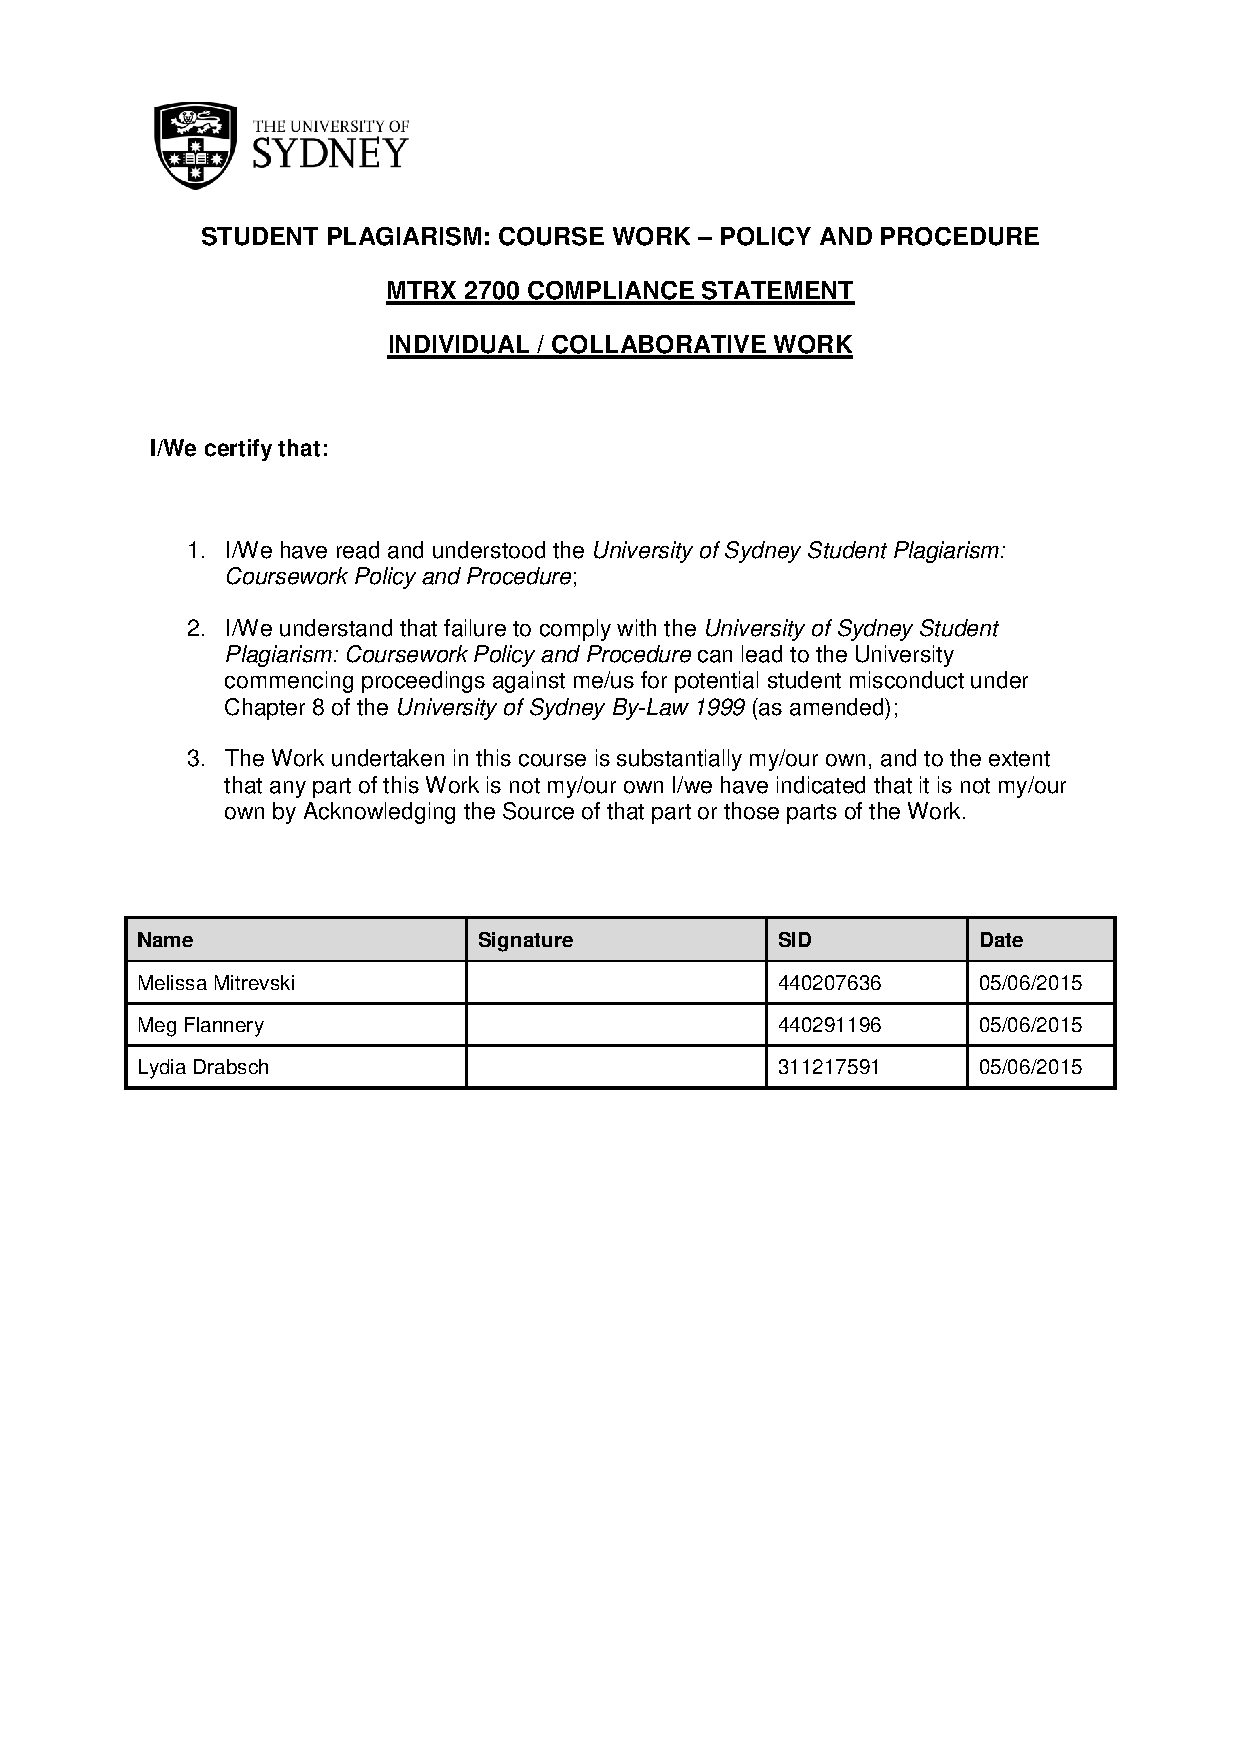
\includegraphics[width=0.99\linewidth]{./Plag}
\label{fig:Plag}
\end{figure*}

%\setcounter{section}{-1}
\section*{Group Certification}
We certify that the design, implementation, and documentation presented by our Group are, unless otherwise acknowledged, the work of our group members only, and that the individuals named below were responsible for completing the following percentages of the modules named.    

\begin{table}[h]
\centering
\begin{tabular}{|p{4cm}|p{0.75cm}|p{5cm}|p{4cm}|}
\hline Name & \% & of the Module & Signature\\
\hline Lydia DRABSCH & & &  \\
\cline{2-3} 311217591 & & & \\
\cline{2-3} & & & \\
\cline{2-3} & & & \\
\hline Melissa MITREVSKI& & & \\
\cline{2-3} 440207636 & & & \\
\cline{2-3} & & & \\
\cline{2-3} & & & \\
\hline Meg FLANNERY & & & \\
\cline{2-3} 440291196 & & & \\
\cline{2-3} & & & \\
\cline{2-3} & & & \\
\hline
\end{tabular}
\end{table}
\newpage

\tableofcontents
\listoffigures
\listoftables
\newpage
\pagenumbering{arabic}
%\renewcommand{\thepage}{\arabic{page}}


\section{Introduction}
\subsection{Document Identification}
This document describes the design of something. This document is prepared by Group ZULU for assessment in MTRX2700 in 2010.
\subsection{System Overview}
A brief statement of the purpose of the system or subsystem to which this document applies.
\subsection{Document Overview}
A short “road map” of the document, to provide an orientation for the reader. Summarise the purpose and contents of this document.
\subsection{Reference Documents}
The present document is prepared on the basis of the following reference documents, and should be read in conjunction with them.\\
—.  “CAN Specification 2.0”.  Robert Bosch GmbH, Stuttgart, September 1991.\\
—.  “OMG Unified Modeling Language Specification”, vers.1.3, June 1999.

\subsubsection{Acronyms and Abbreviations}
Table \ref{Acro} lists the acronyms and abbreviations used in this document.
\begin{table}[h]
\centering
\caption{Acronyms and Abbreviations}
\label{Acro}
\begin{tabular}{|l|l|}
\hline Acronym & Meaning \\
\hline MPC & Model Predictive Control \\
\hline & \\
\hline
\end{tabular}
\end{table}

\section{System Description}
This section is intended to give a general overview of the basis for the something system design, of its division into hardware and software modules, and of its development and implementation.  
\subsection{Introduction}
Give a technical description of the function of the whole system, in terms of its constituent parts, here termed modules. Generally, a module will have hardware and software parts.
\subsection{Operational Scenarios}
Describe how the system is to be used. There may be several different ways that it can be used, perhaps involving different users, or classes of user. Present use case diagrams here if you are using them. Each operational scenario is a part through a use case diagram – a way of using the system, with different outcomes or methods of use. \\
You should also consider the various failures that may occur, and the consequences of these failures.

\subsection{System Requirements}
The operational scenarios considered place certain requirements on the whole something system, and on the modules that comprise it.\\
Statement of requirements that affect the system as a whole, and are not restricted to only a subset of its modules.

\subsection{Module Design}
Describe the breakdown of the design into functional modules. Each module probably contains both software and hardware.\\
Then include a section like the following (2.5) for each module. Not all of the sub-headings may be relevant for each module.




\subsection{Module Requirements: Module X}
The operational scenarios considered place certain requirements on the something system, and on the modules that comprise it.
\subsubsection{Functional Requirements}
This section describes the functional requirements of Module X – those requirements that must be met if the module (and system) is to function correctly.  

\paragraph{Inputs}
Describe each external input, including signal encoding and timing, message encoding and timing, protocols, file formats, protection against input errors, etc, as relevant.
\paragraph{Process}
Describe the internal signal transformations and/or computer processing functionality required within the module, required performance limits, and error tolerances as appropriate.
\paragraph{Outputs}
Describe outputs that must be produced for the module to function correctly, including timing, frequency, protocols, etc as relevant.
\paragraph{Timing}
Any required timing or latency specifications that must be met.
\paragraph{Failure Modes}
Required functionality (if any) in the event of failure of various nominated components.

\subsubsection{Non-Function (Quality of Service) Requirements}
Non-functional requirements do not need to be met for the device to have basic function, but are required to provide specific levels of performance or engineering quality.
\paragraph{Performance}
Requirements such as computational loop time, accuracy, etc.
\paragraph{Interfaces}
Requirements such as computational loop time, accuracy, etc.
\paragraph{Design Constraints}
Practical or commercial considerations, such as programming languages, processor or other hardware, etc.
\subsection{Conceptual Design: Software Module X}
Now, for each module, give the outline of how it will work. In this section it is appropriate to present \\
•	The rationale for the design decisions that were made – why things were designed the way they were\\
•	block diagrams,\\
•	mathematical models and algorithms,\\
•	data flow diagrams\\
•	state-transition diagrams\\
•	listings of input and output formats\\
•	listings of message and data formats\\
•	responses to identifiable error conditions\\
•	responses to identifiable failure conditions\\
as appropriate for each module.

\subsubsection{Assumptions Made}
State any assumptions made.
\subsubsection{Constraints on Module X Performance}
State any constraints that may prevent the design from satisfying its requirements.

\section{User Interface Design}
Give a detailed description of the design of the user interface. This will give the reader a good view of how the system functions from the user’s perspective.
\subsection{Classes of User}
If there are different user interfaces presented to different classes of users, define these user classes, and how access by the various user classes is enabled or disabled.
\subsection{Interface Design: User Class Y}
\subsubsection{User Inputs and Outputs}
Description of how the user presents inputs to the system, and how the system responds to those inputs. Include a description of how the user knows the state of the system.
\subsubsection{Input Validation and Error Trapping}
Describe how the system validates user input, and how operator errors are trapped and can be recovered from.

\section{Hardware Design}
Give a detailed description of the design of hardware. The description should include mechanical drawings, location diagrams, electrical circuit schematics, circuit simulation or test results, PCB overlays, wiring diagrams, connector pinout lists, pneumatic/hydraulic circuit diagrams

\subsection{Scope of the Something System Hardware}
Statement of what is, and what is not, being designed and described here.
\subsection{Hardware Design}
\subsubsection{Power Supply}
Power supply method and rating, fusing, distribution, grounding and protective earth as appropriate.
\subsubsection{Computer Design}
Description of computer hardware, including all interface circuitry to sensors, actuators, and I/O hardware.
\subsubsection{Sensor Hardware}
\subsubsection{Actuator Hardware}
\subsubsection{Operator Input Hardware}
\subsubsection{Operator Output Hardware}
\subsubsection{Hardware Quality Assurance}
Describe any measures that were taken to control (improve) hardware quality and reliability – Heartbeats, brownout conditioning/resets, reset conditions, testing and validation, etc.

\subsection{Hardware Validation}
Details of any systematic testing to ensure that the hardware actually functions as intended.
\subsection{Hardware Calibration Procedures}
Procedures for calibration required in the factory, or in the field.
\subsection{Hardware Maintenance and Adjustment}
Routine adjustment and maintenance procedures.

\section{Software Design}
The software requirements and overview have been dealt with elsewhere in this document. The present section addresses the design and implementation of the software that forms the X system.
\subsection{Software Design Process}
How you went about designing the software – top down, bottom up, OOD, functional view, etc.
\subsubsection{Software Development Environment}
The tools that were used, both software (compilers, assemblers, etc) and hardware (development boards, etc.).
\subsubsection{Software Implementation Stages and Test Plans}
Describe the way you went about implementing the software - staged implementation, pseudocode (PDL), unit testing procedures, integration testing, etc. Identify dependencies – e.g this had to be done before that, etc.
\subsection{Software Quality Assurance}
Describe any measures that were taken to control (improve) the software quality – code or documentation standards, code walkthroughs, testing and validation, etc.

\subsection{Software Design Description}
\subsubsection{Architecture}
Describe the high-level architecture of the software – that is, the top-level flow of control, and how the various functional modules communicate.\\
In this section, you can put state transition diagrams, sequence diagrams, etc.
\subsubsection{Software Interface}
Describe the public interface of each software module.
\subsubsection{Software Components}
This is a detailed view of the internal workings of each of the software modules.

\subsection{Preconditions for Software}
\subsubsection{Preconditions for System Startup}
Describe any preconditions that must be satisfied before the system can be started.
\subsubsection{Preconditions for System Shutdown}
Describe any preconditions that must be satisfied before the system can be stopped.
\section{System Performance}
\subsubsection{Performance Testing}
Give the results of testing conducted to determine the characteristics and performance of the system - memory usage, loop time, system accuracy, repeatability, ease of use, etc.
\subsubsection{State of the System as Delivered}
A statement of your group’s opinion of the conformance of the system with the specification.
\subsubsection{Future Improvements}
Present a prioritised list of improvements to be made in future releases, giving reasons for the improvement and priority rank.

\section{Safety Implications}
By law (NSW Occupational Health and Safety Act 2000; NSW Occupational Health and Safety
Regulation 2001) all employees who design plant, machinery or equipment must identify foreseeable safety hazards associated with the equipment, and then assess and control the identified risks. Although this law does not apply directly to student designs, you should consider it here.



\section{Conclusions}

\newpage
\bibliographystyle{IEEEtran}
\bibliography{file}


\newpage
\section{Appendix}

\end{document}